\documentclass[11pt,a4paper]{article}
\usepackage{natbib}
\usepackage{a4wide}
\usepackage{graphicx}
\usepackage{lmodern}
\usepackage{fullpage}
\usepackage{draftwatermark}
\SetWatermarkText{DRAFT}
\SetWatermarkScale{2}

\pagestyle{plain}
\title{\textbf{Game theory in conjunction with data analysis: a potential tool for health service evaluation and planning.}}
\author{Dr Greig Russell, \\ BSc BMedSc, MBChB, BA, PGDipCEM \\ MAAFP, FRNZCGP, FRNZCUC, FACHI}
		\date{\today}
		
\bibliographystyle{apalike}

\usepackage{graphicx}
\begin{document}
\maketitle
\Large{\textbf{Report for Dr Kenneth Clark, MidCentral DHB}}

\Large{\textbf{Professional Practice (152.894)}}
\newline
\newline
\newline
\begin{figure}[htp]
\centering

\includegraphics[scale=0.6]{PN.png}
\caption{Palmerston North's square at night}
\label{}
\end{figure}

\pagebreak
\section{Executive summary}
This report advocates for the use of Game Theory as another tool for the economic evaluation of reforms within New Zealand's primary healthcare system. The approach adopted is to evaluate the most recent reforms to the funding and delivery of healthcare within primary care using modern data analysis methods, particularly statistical process control and time series analysis. Game theory is used to interpret the results of this analysis in the context of both the intention and the local reality of the policy. The novel application of Games Theory will be shown to develop an extra dimension to understanding the impacts of the health reforms beyond classic "supply \& demand" microeconomic theory.\\

In economics, Game Theory is used to explain or develop a winning economic strategy. All businesses that adopt this optimal strategy flourish or at least survive while those that do not inevitably perish. A strategy can focus on the range of goods or access to the market. In health markets like primary care provision, then the range of products and internal business model is similar to all providers, so the  only variable that can change is the market's ability to access that provider \citep{dinar2008game}. \\

Game theory has been applied to the development of health systems. \citet{dobson2004sustainable}, used the combination of game theory and social network analysis to understand the development of an integrated local mental health initiative. Their study found that the outcome of the initiative for participants was driven by the social network in which decisions were made \citep{dobson2004sustainable}. The analysis was made by analogy to the famous game called the "Prisoner's dilemma", where the players get a moderate adverse outcome through cooperation, while one would receive a favourable outcome and the other a much worse through not cooperating. This study suggested that, by failing to consider how to optimise their position, the participants left themselves vulnerable to the worst case outcom e\citep{dobson2004sustainable}. \\

The two reforms considered were the "2001 Primary Healthcare strategy" \citep{king2001primary} and the "Free primary care for under 13 year" policy\citep{frizelle2014health}.\\

The hope in the "2001 Primary Healthcare Strategy" \citep{king2001primary} was that the delivery of general practice care would move from a doctor-centred, fee for service, acute reactive care model to a capitation funded, multidisciplinary preventative care model. \citet{hefford2005reducing} describes a promising start until the negative reality described by \citet{howell2005restructuring} emerged. The practitioners did not change their business model from a fee for service and remained focusing on competing for the co-payment not competing in an open market for capitation dollars. With time practices reduced in number, as capitation funding caused an effective block to the establishment of new general practices. The survivors, now more affluent that prior to 2001, transformed from an equity model through competition to a retail model of primary health care deliver fighting with other retailers for the disposable income of the affluent. Despite the large injection of funding into primary care following release of the primary care strategy, capitation funding has reduced equity of access. General Practice is now a retailer of heath care provision not the hoped for agent of social equity.\\

The data analysis revealed that from 2001-2016 the general practices in Palmerston North have progressively moved from a position providing equity of access for the city's 'population to a narrow arc through the centre of the city. This arc was found to be similar to the control group of non-government funded retailers. The arc was located at the point of equidistant between centres of affluence in the city. Game theory suggests that this represents the Nash equilibrium for retail provision. Any business not located on this arc is at an economic disadvantage to its competitors, so must move onto the arc or fail to thrive.\\

The second primary healthcare funding reform considered was the "Free primary care for under 13 years" strategy \citep{frizelle2014health}. \citet{schoen2009survey} described how cost was a barrier to care in New Zealand. The atlas of health care variation, developed by the Health Care Safety Commission reports a wide variation in engagement and clinical outcomes for children in New Zealand \footnote{http://www.health.govt.nz/publication/indicators-well-child-tamariki-ora-quality-improvement-framework-september-2014}.To address this level of unmet need, the incoming National government made consultations for children and your people under age 13 free within primary care\citep{frizelle2014health}. \\

Intuitively this makes sense. If is injected more funding, specifically targeted to reduce the barriers to accessing primary care, then young people will access appropriate care and the right time. This will lead to a reduction in terms of preventable mortality or hospital admissions and a reduction in the variation care received across the country. The introduction of this policy, made no impact on General Practice utilisation in the study locality of Palmerston North. Instead the policy apparently triggered an unparalleled utilisation of the hospital ED, but by not the target group. Instead it was adults, often affluent, who went to ED while young people went to Urgent Care clinics. This report would argue the rise is causally elated to the introduction of the "free under 13yrs" funding policy. As seen in the statistical process plots below, the rise coincided temporally with the policies introduction. The rise of 3 standard deviations from the usual mean attendances, outlasted both the seasonal influenza outbreak and the winter surge in general.\\

\citet{howell2005restructuring} described how small group or solo practices lacked the critical mass of patients required to risk manage the utilisation variation required for capitation funding to impact on patients access to care. As described above the economic focus of these small and solo practices was on maximising patient co-payments. Capitation funding was evenly spread between all practitioners, this increase in funding was also spread evenly, so triggered no competitive pressures or opportunities within General Practice owners. Evenly spread changes in capitation funding will have no impact on retail providers focused on competing for a different economic priority.\\

The policy instead appeared to trigger a social change in attitudes towards access care and a perception that health should be provided free at point of care. Urgent care providers were swamped with young people. The Palmerston North Hospital Emergency Department has and continues to experience unprecedented demand. So while the policy has had an effect of the provision of primary health in Palmerston North, it has produced no economic changes in General Practice. Although insufficient time might have passed, there has been immediate shift in the arcs of the Nash equilibrium for primary care providers.\\

So while Games theory appears to be a tool for the evaluation of previous healthcare provision reforms, its ability at prediction needs to be tested. Health has realise the importance of primary care to deliver an affordable, accessible, and effective health service. Indeed this is one of the central tenets of the 2016 Health Care Strategy \footnote{http://www.health.govt.nz/publication/new-zealand-health-strategy-2016}. MidCentral DHB has invested in primary care culminating in the opening across the district of several large Integrated Family Health Care Centres. These centres are amalgamations of smaller 1-4 General Practitioner surgeries and provide care for ~15,000-20,000 patients. Although these have been under development for some time, enough have now opened that most patients across the district will receive their General Practice care through an IFHC.\\


This development may create a paradox. The IFHC that is now large enough to risk manage capitation funding as a basis for funding, allowing capitation funding to become the economic driver that makes care for disadvantaged attractive that it was originally intended to be in the Primary Healthcare strategy \citep{king2001primary}. Indeed capitation funding will be increasingly attractive to IFHC, as growth slows in the co-payment market associated with slow population growth and market saturation for primary care provision to the affluent. The IFHC also face increased cost with new enlarged facilities and the establishment costs of the amalgamations. So while both the need and the opportunity exists, IFHC may struggle to exploit the opportunities.\\

These dilemmas will create economic pressures on existing businesses, so Game theory would predict that the arcs associated with the Nash equilibrium will shift with time. These shifts will reflect changes in IFHC business models including the potential for some to fail if they can not adapt, but also the impact of any new macroeconomic policies or realities will drive shifts. The DHB could base any market interventions it might be contemplating on where they wish those Nash equilibrium arcs to be located in the geographical as well as the economic landscape.\\

There are two limitations to the current study. Firstly the publicly available data was of inferior quality. Secondly this study has also identified how the analysis techniques can be modified to over come the lack of historical data, which was the original driver to use the publicly available data set. The second limitation was the sample size. Palmerston North is not a big enough market to fully consider the impact of Game theory and data analysis methods on health service evaluation and planning.\\

This study did give qualified support as to the possibility, but more research is needed.\\

\subsection{Recommendations}
 
\begin{enumerate}
\item That although this report provides initial support for Game Theory in conjunction with modern data analysis methods as a basis for assessing and planning healthcare delivery, more research is needed.
\item Specifically the study needs to be repeated in another and larger market.
\item The study needs to be repeated with a more robust and comprehensive data set.
\item The study needs to be longitudinal given the long time frames for changes within primary care impacting on the business models of owners.
\item MidCentral DHB needs to consider how it will meet the needs of the disadvantaged or those that live in areas of high need. Consideration may be given to opening a medical centre in such an area. It will be important that barriers to capture by the affluent are set in place. If the health centre was a welfare centre established as a joint venture with Ministries of Housing \& Social Welfare then the rules of the "game" would be different from those seen at the IFHC or General Practices within Palmerston North.
\item MidCentral DHB needs to consider changing the paradigm of primary and secondary care being separate entities. Events in once cause negative impacts in the other. These issues can only be addressed through adopting a whole of sector management strategy. 
\end{enumerate}
\pagebreak

\tableofcontents

\pagebreak
\pagebreak

\listoffigures

\pagebreak
\section{Introduction}
Primary care delivery within the MidCentral District Health Board (MDHB) region is currently undergoing its biggest change since the introduction of capitation funding and the associated shift to population health from the previous "fee for service" funding model.\\

There has been a district wide drive to amalgamate small practices into larger Integrated Family Health Centres (IFHC), where groups of ten or more doctors, plus their associated nursing staff provide primary care for blocks of  15,000-20,000 patients. This is the third major reform of the local primary care health sector in the last 15 years and the second in the last two years. Both of the previous reforms were changes in national health policy, while the development of the IFHC, although also a national program required considerable local support by the MidCentral District Health Board (MDHB) for it to occur. \\

This report will investigate the use of Game Theory to interpret the analysis of the data describing the impacts of the previous two reforms, namely the move to capitation based funding and providing free care to all aged under 13 years. This report investigates the impacts of the previous two reforms and describes the relationship between their actual impacts and the original policy intent. If Game Theory can offer explanatory benefit to that relationship, it could be the basis for future service planning and evaluation of the impacts of previous policy initiatives.\\ 

The previous national health funding reform was when on the 1st July 2015, the incoming National government implemented its election promise to make care free for all children aged 6-12 years who were registered with a Primary Healthcare Organisation (PHO)\footnote{http://www.health.govt.nz/your-health/services-and-support/health-care-services/visiting-doctor/zero-fee-doctors-visits-children-aged-under-13}.\\

For primary health care providers, the focus was about getting adequate compensation to offset any income loss\footnote{http://www.radionz.co.nz/news/political/271689/doctor-visit-promise-falls-short}. Within the secondary care environment, little comment was heard. This funding change was only seen as impacting primary care and even then in a marginal sense.\\

What happened was totally unexpected, as this reform seemed simple, almost administrative, and clearly aimed at only General Practice. Instead of more patients  attending their General Practitioners, locally patients flooded both the local community based urgent care clinics and the hospital Emergency Department. The record numbers attending acute services have now become the new normal, but this is placing pressure on unchanging hospital budgets. \\

This unexpected result to a "minor" funding change was contrary to what was expected under the Primary Health Care strategy when it was released by the then Minister of Health, Annette King \citep{king2001primary}. As envisaged, the "free under 12 years" funding shift should have lead to better access to primary care by the 6-12 year old age group because it further reduced the financial barriers to accessing care. The intention of the 2001 reforms was to move away from reactive, fee for service care delivered by only doctors. Instead care would be multidisciplinary teams focusing on the health of the entire population and focusing on wellness not illness \citep{king2001primary}.  The need then is to understand the impacts of the primary health care strategy on primary health care delivery so as to be able to understand what caused the paradoxical effects of extending the scheme in July 2015.\\

This report will use analysis techniques like statistical process control to understand the operational flows within the emergency department \citep{rosemann2015six, cheng2015run, epprecht2015statistical}. Statistical process control technqiues have already been used to study the operational function of emergency departments \citep{pimentel2015statistical} and are widely used within the field of quality improvement \citep{provost2011health}.\\

Previous internal studies on the utilisation of the Emergency Department had noted a marked geographical maldistribution. This result was unexpected, except by the Emergency Department staff who had known it all along. They assumed everyone else also knew. To consider the impact of geography on the health system and consumer behaviour, Geospatial Information System (GIS) and Games Theory analysis techniques were used.\\

\section{Literature review}
\subsection{Game theory}
In economics, Game Theory is used to explain or develop a winning economic strategy. All businesses that adopt this optimal strategy flourish or at least survive while those that do not inevitably perish. A strategy can focus on the range of goods or access to the market. In health markets like primary care provision, then the range of products and internal business model is similar to all providers, so the  only variable that can change is the market's ability to access that provider \citep{dinar2008game}. \\


This analysis will use the concept of a "Nash equilibrium" to underpin the understanding of the Graphic Information Systems data. This is the position adopted by two players in a non-cooperative or competitive game. The key concept is that this is the position (frequently geographic) that no-player is worse off for adopting. This is not say that any one player might not be better off for adopting another position at the cost of the other players. The position of the Nash Equlibrium is position where no player is worse off than any others.\\  

To demonstrate this concept, the most frequently used example describes two ice cream vendors on a beach. The first sets up in the middle of the beach and gets unique access to 100\% of the market. With the arrival of the second, the profit-maximising position for them both on the beach is for one to be at 25\% along the beach and the other at 75\%. The reality is both will be found in the middle, with both ice creams vendors beside one another selling the same goods at the same price. Game theory predicts this because if one vendor suddenly moves to the middle of the beach, then they will control 75\% of the market, a considerable gain. The other vendor, who stayed still, will only control the other 25\% position. The profit maximising position may therefore create the most profit, but also promotes the most risk. If both move to the middle, neither can lose a share of the market to the other and so this is the position where neither can lose from the actions of any one else, and no party consistently gains by moving away from it. The middle position, which minimises the risks to all players, or the position of no regrets is called the Nash Equilibrium. In a stable, mature market, the geographic position of business clusters is described as  the Nash Equilibrium between the economic forces under which the businesses operate. If two groups of businesses have similar Nash equilibrium positions as seen from geographic locations, then they operate under similar economic forces. If they are in different locations then the two sectors are reacting to various economic drivers. \\

Game theory has been applied to the development of health systems. \citep{dobson2004sustainable}, used the combination of game theory and social network analysis to understand the development of an integrated local mental health initiative. This study found that the outcome of the initiative for participants was driven by the social network in which decisions were made. The analysis was made by analogy to the famous game called the "Prisoner's dilemma", where the players get a moderate adverse outcome through cooperation, while one would receive a favourable outcome and the other a much worse through not cooperating. This study suggested that, by failing to consider how to optimise their position, the participants left themselves vulnerable to the worst case outcome. \\

The "Prisoner's dilemma" is an example of a cooperative game \citep{binmore2007}. In contrast to the "Nash equilibrium" which does imply any relationship between the players, the "Prisoner's dilemma" implies some form of underlying relationship which underpins the game \citep{binmore2007game}. The classic description of the dilemma is two criminals, equally guilty, who have been caught. Each is held independently and made an offer. If they both stay silent, they both get one year in prison. If they provide evidence against the other, they will be set free but their "friend" will get a longer prison term. From the Social Network analysis performed on this data set, no evidence of cooperative behaviour was found. For this reason the analysis was based on the "Nash equilibrium", which does not have the requirement for cooperative behaviour, in fact this is a specific exclusion. \\

\citet{tarrant2010continuity}, have used Game Theory to understand the drivers behind patient trust of primary care physicians and how that changes with time. There were difficulties previously in understanding engagement, whether long term relationships lead to the evolution of trust in primary care physicians and if so, the reason behind this development. The authors' use of Game Theory enabled them to describe the underlying "game" of the therapeutic relationship. They found that patients started from a position of the generic physician encounter based on a social construct of the generic physician consultation. Game theory predicts that by repeated individual encounters, mutual benefit from the relationship develops as both seek insurance against "the shadow of the future" \citep{tarrant2010continuity}. Each participant makes no assumption of each others motivation. Indeed ill health is the shadow for the patient while financial insecurity or clinical medico-legal risk  are drivers for the physician. Game theory predicts that even without any shared motivations the optimal position for both is the development of a long term relationship to address clinical problems.  This study is not testing Game Theory but is using Game Theory to understand a social phenomenon. \\

\citet{chapman2012using}, used Game Theory to investigate incentives for uptake of annual influenza vaccinations.  The study found that when the incentives reflected self-interest the older group of players got vaccinated while the younger group did not. When the incentives were changed to reflect outcome for the total community (a "get vaccinated to protect your grandmother" style approach) the new Nash equilibrium position reflected a group-optimal utilitarian position. This study again used Game Theory to understand clinical behaviour in the community. It also showed the use of Nash equilibrium to illustrate changes in the net position of a population of non-cooperating individuals. \\

Game theory is in one respect an emergent economic theory, yet it is also an established theory, with an increasing repertoire of useful applications in different situations. \\

\subsection{Evaluation of previous primary care reforms}
With the election of the fifth Labour government in 1999, Minister King had inherited a health system that had been through a series of minor changes, but which had remained, from a patient perspective, for many decades. Until the early 1990s, the New Zealand primary care system had been one of a state subsidy based on a fee for service by a doctor \citep{gauld2006new}. For providers there had been considerable changes over the 1990s. With the neo-conservative health reforms of the early 1990s a split between the funders of health and the providers of care was introduced. The aim was market driven efficiency's of care provision through providers competing amongst each other. General Practitioners were allowed to form Independent Practitioner Associations (IPA) so as to form groups of sufficient size to improve the ability of General Practices to participate effectively in a competitive health care market, including with hospitals both public and private. These IPA continued to be predominantly GP led and, as organisations, they remained primarily focused on protecting their General Practitioner members from any negative impacts of the neoliberal health reforms \citep{malcolm1999new}. Some IPA achieved successes through profit sharing arrangements with the new funding bodies, but essentially from a patient perspective it was business as it had always been. The Government funding of primary care provided less than 10\% of income during practice in this era. This percentage of practice income provided by the state to subsidise patient fees and ease access to community based health care was reduced each year. As the rate of inflation was greater than the rate by which the subsidy increased, the subsidy became an increasingly smaller component of practice income. Even this seriously limited subsidy applied only if the doctor saw the patient and did not apply if the patient saw the practice nurse or other staff member. \\    

The Primary Health Care Strategy wanted to achieve a more fundamental reform of primary care and had broader aims \citep{king2001primary}. Under the strategy, health care was to be about the health of entire populations and focused on providing this preventive health care delivered by multidisciplinary teams. The funding of primary care was to be on a capitation basis where subsidies to practices were on a fixed income per annum per enrolled patient and not on an activity basis. It was in a practice's financial interest to spread consultations across all team members as this improved profitability by increasing the number of patients the practice could enrol, so maximising the practice income. Only by focusing on preventive health care could the required reduction in consultation rate per patient be achieved, given fixed annual subsidy per patient per annum. The intention of the strategy was this combination of larger practice sizes and preventive care delivered by multi-disciplinary teams. By this means, New Zealand would achieve both population health at the same time as improving primary care profitability\citep{king2001primary}.\\

The shift to capitation-based funding also removed the funding barrier to non-medical providers participating in health care provision. Indeed, a fixed income should have encouraged practices to use cheaper nurses to provide patient care than more expensive doctors whenever possible. It was imagined that nurses could open their own practices without doctors, so expanding the range of providers, increase competition and so drive down patient costs through classic economical "supply \& demand" theory. Also envisaged in the strategy, was that all professional groups could now contribute to overall community health outcomes, with each team member working at the top of his or her scope of practice.\\

Driving the adoption and success of the new strategy was an increase in overall health funding of \$500 million per year from 2002-2008 \citep{gauld2006new}. Increased demand for health care, especially in areas of deprivation, was to have been driven by this dramatic increase in funding \citep{king2001primary}. The general practices would remain independent businesses, usually owner operated. Service provision was to be delivered via a series of contracts, only one of which is for the provision of primary medical care in the community with Ministry of Health. Under the strategy the previous physician dominated "Independent Practitioner Associations" (IPA) became "Primary Healthcare Organisations" (PHO). The nature of the contracts allowed the practices to effectively ignore the PHO if they wished. The funding is transferred from Ministry of Health to individual practices via the DHB and local PHO\footnote{http://www.health.govt.nz/our-work/primary-health-care/primary-health-care-services-funding-and-contracting}. The contracts themselves are national contracts between the NZMA and the Ministry of Health\footnote{http://www.nzdoctor.co.nz/news/2016/may-2016/16/increase-of-1-per-cent--in-capitation-proposed-for-general-practice.aspx}.\\

The Primary Health Care Strategy aimed to establish a local free marketplace, with funding to enable all patients to participate as they sought the best deal from multiple suppliers or practices. Patient demand was to drive primary health care to the optimal allocative efficiency of resources to meet their health care needs. It was envisaged, moreover, that the behaviour of the primary health care market in a given locality would be regulated automatically by the 'invisible hand' or inherently self-regulating nature of a free market. In this situation, the focus of the Government was to be on ensuring participation of those from areas of deprivation and poverty. \\

The challenge in this field of study, has been how to evaluate the actual impacts of the strategy on society and the health system \citep{howell2005restructuring}. Studies considering the impacts of the Primary Health Care Strategy \citep{king2001primary} have produced conflicting responses to date. \citet{hefford2005reducing}, examined the strategy's results 15 months after implementation. The authors described the development of performance indicators to allow any effects of the strategy's introduction to be tracked, especially with regards to correcting inequities. The study described  how this increased funding was cumulatively supplemented for those living in areas of high social deprivation by an additional 20\% per enrolled patient in a practice, and by another 20\% for every self-identified Maori or Pacific Islander, who enrolled (p. 14) in the practice \citep{hefford2005reducing}. One clear intention of the strategy was to shift these groups of patients from being financially undesirable to being financially highly desirable. This shift would attract providers to areas of high need and hence correct long-standing health inequities to exploit this new opportunity. If the total enrolled population of ethnic minorities and those who lived in areas of high social deprivation was above 50\% of the locality's enrolled population then further funds were provided to every practice in the locality. \citet{hefford2005reducing}, found that those most in need had enrolled in greater numbers than the general population. The overall level of funding that these ethnic minorities and those patients from socially deprived areas  received was 25-60\% higher under the strategy than under the previous funding formula. The authors argued that this reduction in the cost of care and the observed greater uptake of health care would lead to improved health outcomes for a group of patients previously labelled as undesirable. The authors described overseas studies which found this exact effect \citep{hefford2005reducing}.\\

\citet{howell2005restructuring}, was less optimistic than Hefford. She argued that the strategy is the adoption of an insurance model where the individual practice in effect becomes an insurance agency, where the capitation is a premium that pays for a fixed quota of care. For Howell, once the quota of care is exceeded by the patient, the risk of the financial cost of ill health is transferred to the practice. She identified two groups of patients who will use excess care as compared their capitated funding and so create financial risk for the practice. The practice will then (probably) mitigate that chance by passing the costs of excess use back to the patient through fee rises to all patients.\\

Her first group was the worried well, who may seek more care than their capitation funding allowance, attracted by the reduction in prices. The second group who might care above their capitation funding was those patients with a chronic illness, especially those with multiple comorbidities, attracted by lower prices to get necessary care. The amount of care sought again is in excess of the capitated allowance.\\  

To manage these financial risks the patients fees would rise, especially within a small cohort of patients, such as the 1-3 doctor practice. As spreading the risk of the few across a large cohort of patients would powerfully mitigate these potential risks, Howell argued that any fee rises have adverse effects on the effectiveness of the Primary Health Care Strategy. The affluent, given their greater weekly income, would experience against a background of higher disposable income as only a relatively small reduction in fees affordability. Any fee rise would have a disproportionate effect for poorer people, though, given their initial lower weekly income, so once again fees would act as a barrier to those seeking appropriate care. These increasing costs would act as a disincentive particularly for the preventative care of those with chronic illness and need more frequent attendances to achieve maximal outcomes.  \citet{howell2005restructuring} described how, in order to prevent fees rising, the then Labour government would have had to restrict the historical right for General Practice to control their charges independent of external regulation and change the historical fundamental business model of General Practice away from individual ownership to a collective.  The Labour government was unable to achieve either change.  \\

For \citet{howell2005restructuring}, then, after an initial period of readjustment the patient costs would rise, and the focus of General Practice would remain on those who can afford to be sick. Howell argued for the adoption of an actual insurance model. If such a model was adopted, then the financial risk of chronic illness and the ability to manage locality derived utilisation patterns would be carried by a much larger group of patients and providers than was achieved under the Primary Health Care Strategy by 2005. This would reduce the drivers towards fee increases and its associated distortions to the system.\\

Depressingly, more recent evidence seems to support Howell's pessimism rather than Hefford's optimism when considering the potential of the strategy to achieve its goals of reducing health inequity within the population by providing equality of access. \citet{jatrana2009primary}, described the impact of the strategy on primary care utilisation. Those with the greatest number of current comorbidities, current smokers, those who felt their health was poor, those who had limited education and those who came from the most significant levels of social deprivation - were all likely to delay seeking medical review and were much more liable to delay filling a prescription.  As an example, consumers who were in the NZ Index of Deprivation of 5 or higher were 18.01 times more likely to delay seeking medical review as compared to the lowest group in the NZDep and 24.47 times more likely to delay filling any prescription. \citet{cumming2008reforming}, considered  that although the Labour government was injecting considerable extra funding each year under the strategy, this increase of financing was not passed on as fee reductions.  In fact, by 2005, patient charges, rose on average for adults by 18\% (or \$4.30 / consultation). In practices with the higher levels of social deprivation and large concentrations of ethnically disadvantaged patients, the fees dropped by 20\% (or \$4.40 / consultation) for adults. This reduction represented a small percentage drop in overall household weekly income, militating against its effectiveness in reducing health equity.  The authors described how the most significant impact of the rise in health funding during the implementation of the strategy was the 58\% increase in GP income from \$97,220 to \$153,886 \citep{cumming2008reforming}. This growth in practitioner income together with overall patient fee rises supports Howell's opinion that the GPs continued to manage income from fees as they had done previously, without adopting a managed risk approach, and that they continued to use fees to manage fiscal risk from chronic illness. \\

\citet{howell2005restructuring} prediction was that fees would again become the primary economic driver for the financial stability of practices. Driven by the ageing  population, there would an associated projected rise in the number of patients with chronic illnesses and multiple comorbidities that would lead to an increased  average utilisation rate greater than that provided under the capitation funding rates. The increased government funding provided through the initial roll out of the Primary Health Care Strategy would have offset the impact of increased utilisation on practice income. After the annual growth in funding ceased then the percentage of income from capitation would have to fall as a percentage of total practice revenue, and a rise in the fees derived income would be needed to offset that reduction in the face of rising utilisation.\\

\subsection{Data analysis techniques}
New methodologies for studying such problems have become locally available with the arrival of new (or at least new within the DHB) analysis programs and statistical analysis methods. Although first developed at Auckland University\footnote{https://en.wikipedia.org/wiki/R\_(programming\_language)}, R statistical language has evolved to becoming accessible to non-expert statisticians. \citet{khoury2014big}  describe the hope that with advanced data analytic techniques,  novel predictive hypotheses can be generated from new large data sets so opening up new approaches to patient care. Data is transformed through the use of high level data analysis applications like SAS or R and through the use of techniques like statistical modelling, data mining or machine learning. These tools can manage both the scale and complexity of very large data sets, so allowing the development of the hoped for novel clinical or organisational insights \citep{reshef2011detecting}.  More recently the potential to be found in data analysis within health care, has also been embraced in the newly released revamp of "New Zealand Health Care Strategy" \footnote{http://www.health.govt.nz/publication/new-zealand-health-strategy-2016}. \\

\subsection{Research question}
Formally this report considers the use of statistical data analysis tools, interpreted through the lens of Game Theory to understand the local impact of the "Primary Health Care Strategy" and the "Free care for under 13 years" policy. \\ 

Where Game Theory predicts that businesses will be rationally driven to be located at their Nash equilibrium position for a given set of economic drivers underpinning any macroeconomic policy shift. \\

\pagebreak
\section{Method}
Palmerston North is effectively a geographically isolated city in the mid central of the North Island, at least as far as access to medical care(Figure 1). It is the regional hospital for the provision of cancer treatment services, and usually nearby provincial areas refer to Palmerston North Hospital. The nearest tertiary hospital is approximately two hours drive away, which when considering illness and health care is an impractical distance.\\

\begin{figure}[htp]
\centering
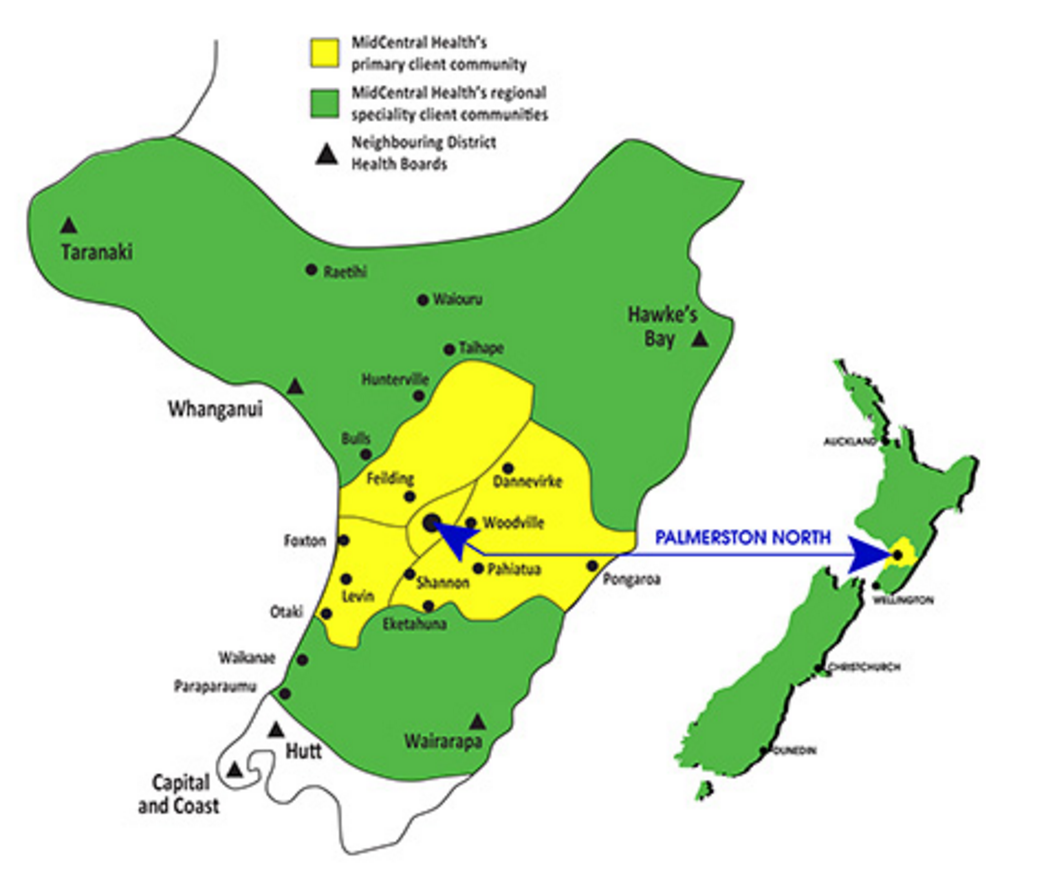
\includegraphics[scale=0.5]{fig1.jpg}
\caption{The location in New Zealand and the total area of responsibility for MidCentral DHB}
\label{MidCentral District Health Board}
\end{figure}

Conveniently Palmerston North is laid out as a rectangle (Figure 2), with deprivation traditionally believed to lie in equally distinct quadrants.\\

\begin{figure}[htp]
\centering

\includegraphics[scale=0.20]{fig2.png}
\caption{The traditional view of the economic layout of Palmerston North. The poorest sector is the top left quadrant, the richest in the bottom right. In between lie the middle classes.}
\label{Traditional view of the spatial economics of Palmerston North City}
\end{figure}

To study the shift in geographical location of practices over time, access to previous practice data was required. The introduction of the primary care strategy led to the disestablishment of the previous General Practice governance structures. This in turn resulted in the loss of all data prior to the disestablishment and this was an unforeseen complication in this study. On review of the options for historical information, the assumption was made that commercial organisations, including medical practices, generate business by advertising. As part of advertising, the address is also supplied along with the nature of the business. Telephone directories are public information, and are held in the local public library. These served as the basis for the geographic data set used in this study.\\

The data collected was simply a table of names of practitioners, the address they gave in the telephone directory of the year and the nature of their practice (solo vs. small group practice vs. large group practice with over five practitioners at a single location,  General practice vs. Urgent care vs. Specialist Care). Only the  medical practices listed in the specialist medical practitioner section of the telephone directory were included. The current government is encouraging the formation of large integrated family health centres. As a byproduct of this further development, the intended location and nature of practices is also known in 2016.\\

Difficulties with using the telephone directory as a data source were immediately apparent, including, for example, occurrences such as a failure to update addresses when practitioners moved to new premises. It was, in addition,  impossible to determine whether there were omissions from the directory. Some group practices only list their medical director, not all medical and nursing staff employed there. As a consequence, the contribution of such practices to the overall provision of health care will be under estimated.  After discussion, it was decided to proceed with the limitations in the data set as no better data set was available.  \\

It is important to have a control group as clearly there are many interdependent factors in any given market that will impact on economic activity by retailers, independent of macroeconomic policy for niche markets like health. A classic example is the 2009 global financial crisis that affected all business including health. To control for these local or global effects on the whole local market, retail alcohol outlets were chosen.  This group was selected as they provide services of similar cost, with similar hours of operation but are not subsidised by central government. Only those hotels, retail alcohol outlets and bars in the relevant sections of business section or "Yellow pages" were considered to be part of this control group. There were similar limitations in the data with regards to this group as there were for medical practitioners. During the time frame considered in this report no changes in national policy occurred.\\

The analysis method comprised of two phases. The first was to use GIS to plot the changes in the geographic distribution of General Practices and retail alcohol outlets in Palmerston North city from 2002 - 2016. The second phase was to try to understand the distribution and changes over time against controls or alternative possible hypotheses. \\

Analysis was carried out using two tools. The network analysis and Heat maps were completed using Google Fusion tables, while the statistical analysis and visualisation of the results were completed using Google Sheets. The Graphic Information System analysis was completed using Google maps. All data was held in a secure data repository that is compliant with FISMA, ISO 27001, ISAE 16/3402 and HIPAA international standards for health data storage. In dealing mathematically  with the inherent issues in this data set, it was treated as a sample not a population. This adjustment partially compensated for the data quality issues. Classical microeconomic theory and game theory was used to consider the results of the GIS study from an economic perspective. \\

Local ethical approval for this study was obtained via the MidCentral Health Clinical Board. The Clinical Board is responsible for all local Health research undertaken within the District Health Board, including primary care.  Regional approval from the Central Health \& Disability Ethics Committee (HDEC) was not required as this study was deemed to be  a low or minimal risk. Massey University ethical approval was granted via generic application by the course convener for 152894 \& 114895. \\

\section{Analysis}
\subsection{2001 primary care reforms}
For Game theory to have any applicability in a GIS based study there has to be geographical movement of practice location. Locally individual practices are, however,  noted for their longevity of location. Social network analysis revealed that General Practitioner turnover was greater than perceived in Palmerston North, despite the prevailing perception being focused on difficulties of attraction not retention (Figure 3). Where social network analysis is a technique that graphically describes the relationship between (in this instance) two variables such as which practitioner was present at a given time.\\

\begin{figure}[htp]
\centering
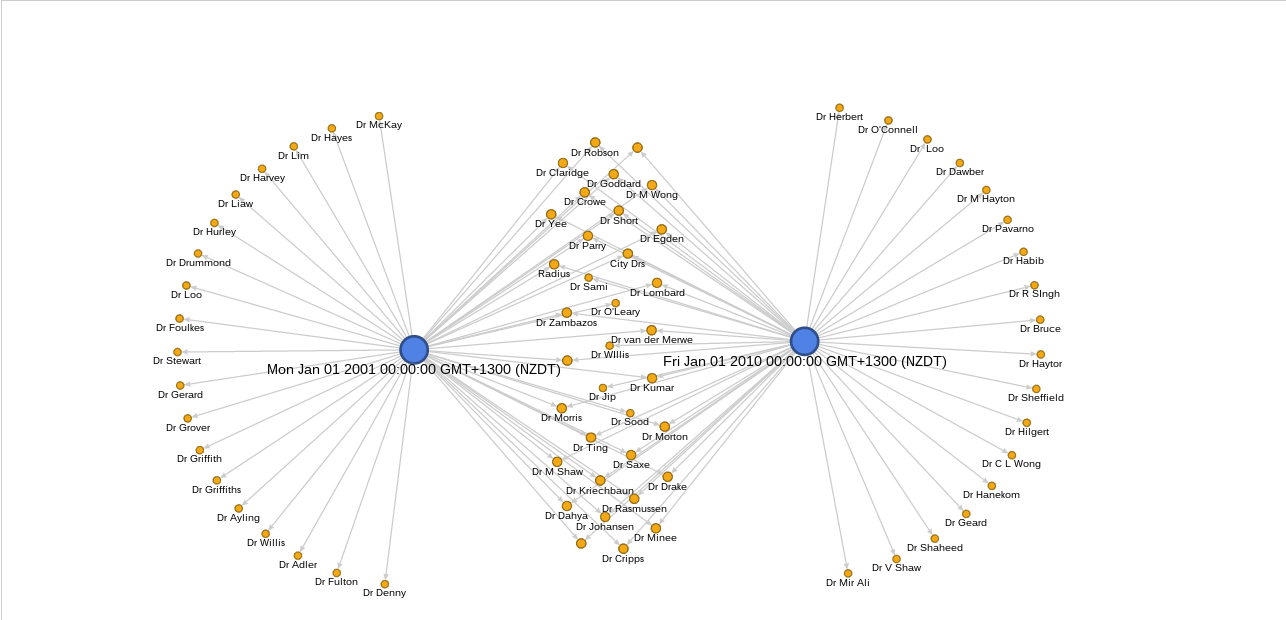
\includegraphics[scale=0.4]{fig3.png}
\caption{Social network analysis showing General Practitioners present in 2002 and 2010, with the group in the middle present at both}
\label{General Practitioners present in 2002 and 2010}
\end{figure}

This turnover of practitioners was the mechanism of practitioner migration within Palmerston North. Where practitioners start new businesses, they open them at perceived better locations as compared to the previous practice location where the business failed to thrive. This makes new General Practitioners rational players in game theory, where rational means making consistent decisions based on maximising their economic benefit. \\

The raw results of the telephone directories and projections for 2016 revealed a far from stable population of practitioners: there is a diminishing population of providers in Palmerston North. There is a core group of practitioners who are pivotal to the stability of supply through their longevity in their practices with a wider group of assistants or transient practices supplementing primary health care delivery. That this group is starting to approach retirement is one of the drivers to establish integrated family health centres, so as to provide a vehicle for succession planning. This reduction in the number of practices is in contrast to the ambitions of the Primary Health Care strategy, one of the aims of which was to increase access through practitioner diversity.  \\

To consider geographic movements of General Practice over time, a series of heat maps was developed from the 2001, and 2016 data respectively.(see figures 6 \& 7). Where the intensity of the flare at a given location is proportional to the number of practitioners at that location.\\ 

\begin{figure}[htp]
\centering
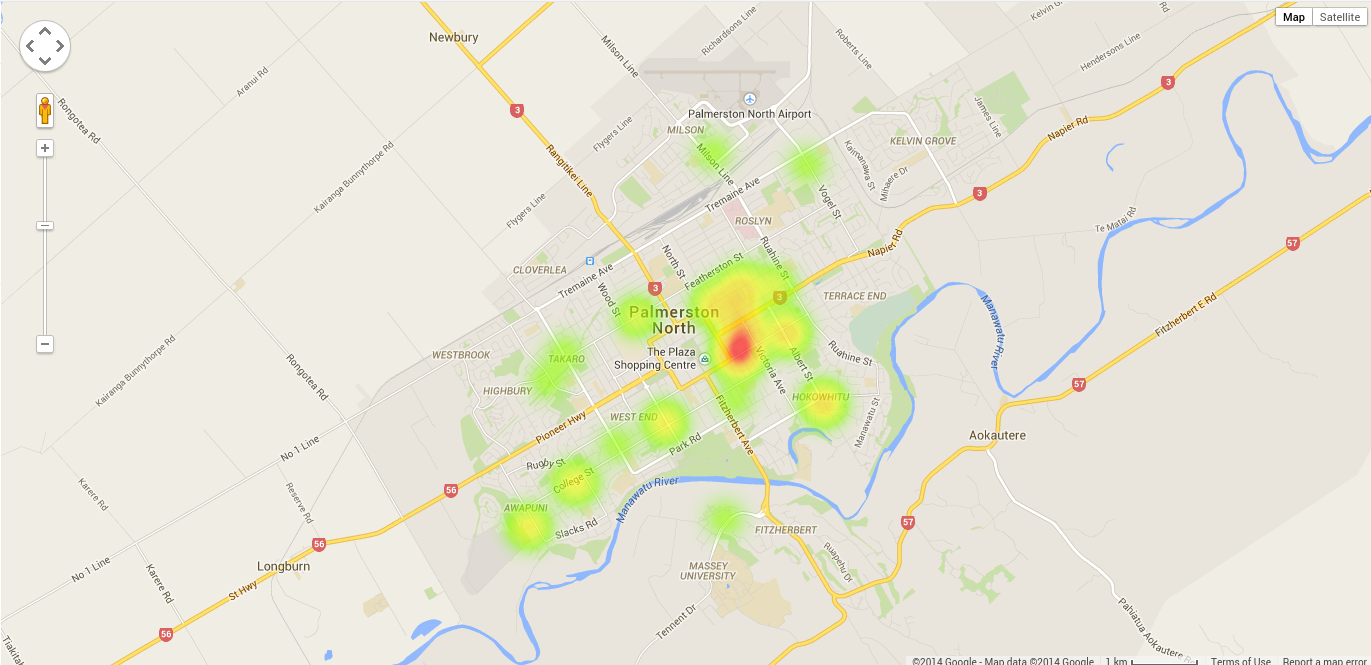
\includegraphics[scale=0.3]{fig6.png}
\caption{Heat map of the distribution of primary care provision within Palmerston North 2001.}
\label{Heat map of practitioners 2001}
\end{figure}  

\begin{figure}[htp]
\centering
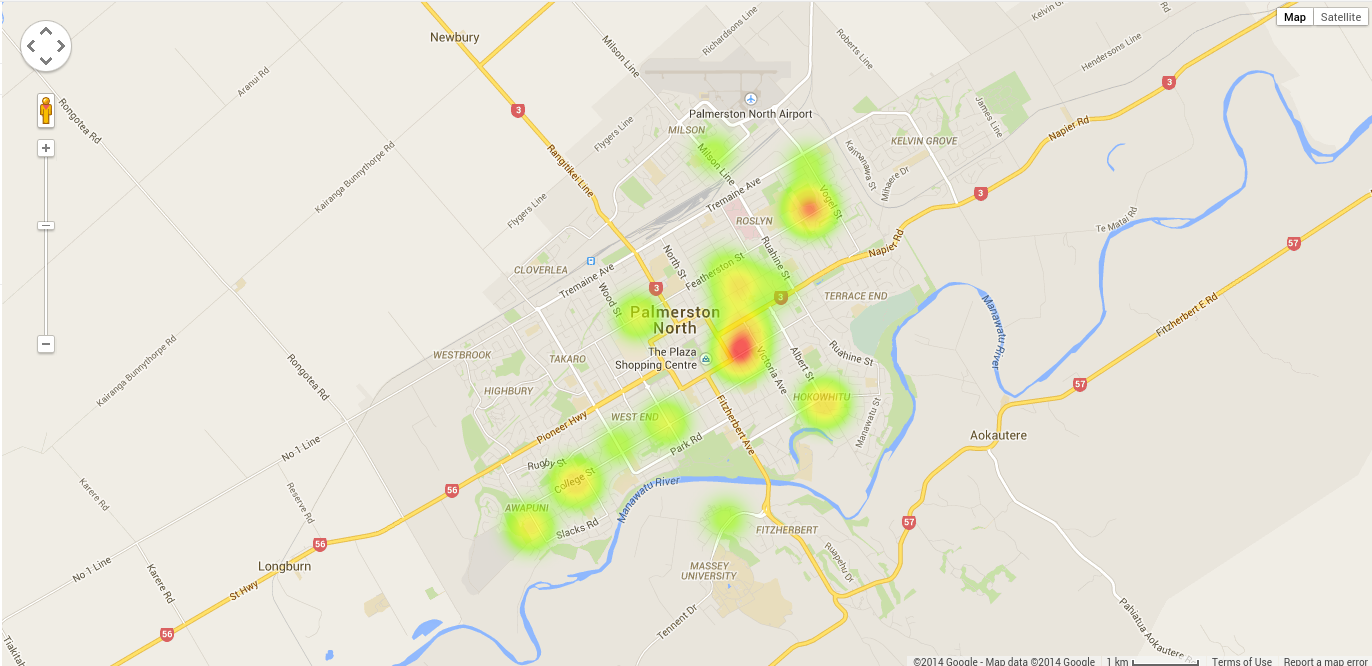
\includegraphics[scale=0.30]{fig7.png}
\caption{Heat map of the projected distribution of primary care provision within Palmerston North 2016}
\label{Heat map of the projected distribution of primary care provision within Palmerston North 2016}
\end{figure}

The map of a sample of patients who presented to ED in 2015 without a current General Practitioner (Figure 8) does not suggest any relationship between.\\

Figure 7 reveals one marker of unmet clinical need. This figure maps the distribution of patients who presented to the Palmerston North Hospital Emergency Department without a current General Practitioner. These are evenly distributed across the city, while practice location is becoming geographical more confined. \\

\begin{figure}[htp]
\centering

\includegraphics[scale=0.30]{fig8.png}
\caption{A sample of 1000 patients who attended Palmerston North Emergency Department,and did not have a GP in 2014}
\label{Distribution of patients with a General Practitioner}
\end{figure}

This distribution of General Practice providers is also quite different from services which aim to achieve equality of access across the town, such as the local bus service (Figure 8). There are, moreover no town planning barriers to the opening of new practices in the suburbs. \footnote{Palmerston North District Plan, R 10.8.1.4}  \\

\begin{figure}[htp]
\centering

\includegraphics[scale=0.3]{fig9.png}
\caption{Distribution of bus routes designed to maximise social equity and access by the public}
\label{Bus routes designed to maximise equity of access}
\end{figure}

\begin{figure}[htp]
\centering
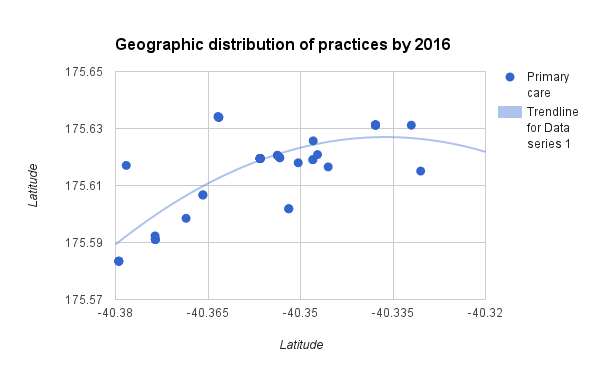
\includegraphics[scale=0.6]{Nash_GP_2016.png}
\caption{Scatterplot of General Practitioner location 2016, with a clear trend line present}
\label{Scatter plot of General Practitioner locations}
\end{figure}

The scatter plot of practice location by latitude and longitude emphasises that there is an underlying central relationship underpinning practice location (Figure 10). Figure 11 emphasises that this relationship also applies to the location of retail alcohol outlets, both in terms of its existence and location within the economic landscape.\\

\begin{figure}[htp]
\centering
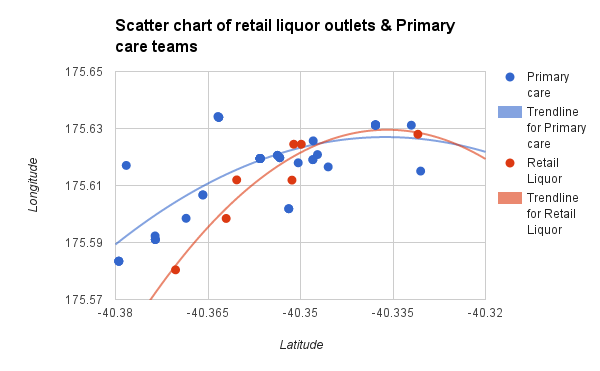
\includegraphics[scale=0.6]{Nash_GP_retail.png}
\caption{ Scattergram of both retail alcohol outlets and Primary Care providers in Palmerston North 2016}
\label{Geographic distribution of practices by 2016, with retail outlets overlaid}
\end{figure}

The distribution of both primary care and retail outlets appears to be maximised in the space between the two areas of affluence within Palmerston North (see figure 12).\\

\begin{figure}[htp]
\centering
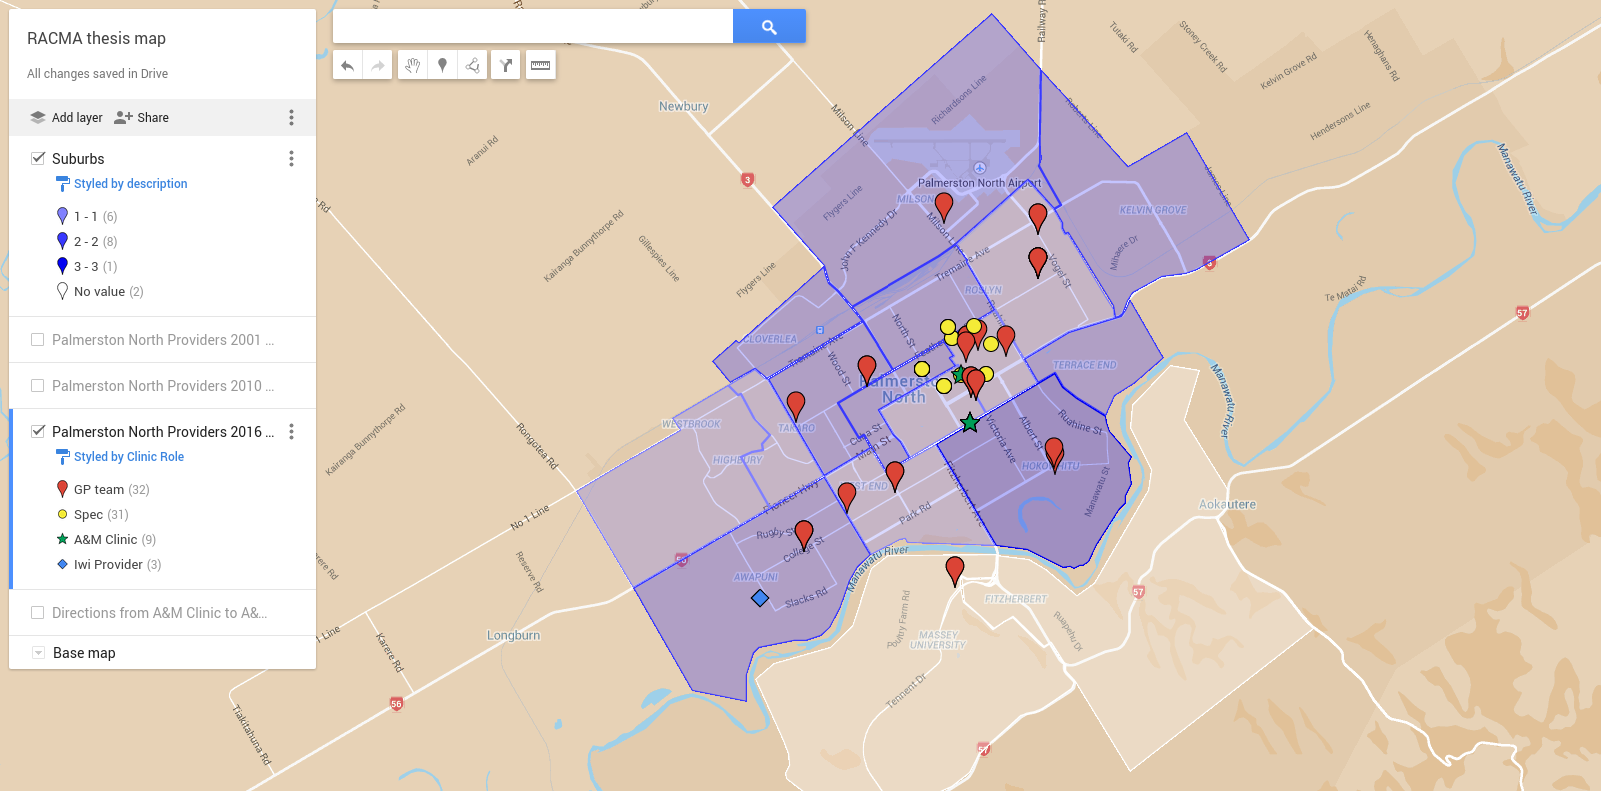
\includegraphics[scale=0.30]{fig12.png}
\caption{The distribution of both primary care and retail outlets appears to be maximised in the space between the two areas of affluence within Palmerston North.}
\label{Distribution of General Practitioners overlaid on suburb's social deprivation}
\end{figure}

\pagebreak
\subsection{2015 "free care for under 13 years" policy}
Following on from the above argument, by 2015 General Practice moving to an activity driven funding model to adopting a retail service delivery model under the guise of the capitation funding model seemed to have no significant adverse effects.\\

Having won the 2014 election, the National Government proceeded to enact its manifesto promise of making the primary care for children aged six to 12 years free at point of care. This extends the age groups full funded to being birth to age 12. Funding and care arrangements for everyone 13 years and older remained the same. The scheme was listed as voluntary and opt-in, 100\% of local providers were participating by the 1.July.2015 launch date.\\

The changes to funding for children aged 6-12 years, then represented a test for the previous model of General Practices becoming a retail outlets competing for disposable income of the affluent. If this model was true, then the impact of changing the capitation payments would have little impact on practitioner behaviour. The changes would impact all practices equally, so not drive behaviour and the economic focus would remain on the patient co-payment.\\

Equally if the original model under the primary health care strategy was correct, then this would be a tremendous opportunity to engage with another group of the population, now freed from financial barriers.\\ 

\subsection{Impacts within General Practice}
The 1.July.2015 launch coincided with the commencement of the annual influenza like illness epidemic (Figure 12). \\

\begin{figure}[htp]
\centering
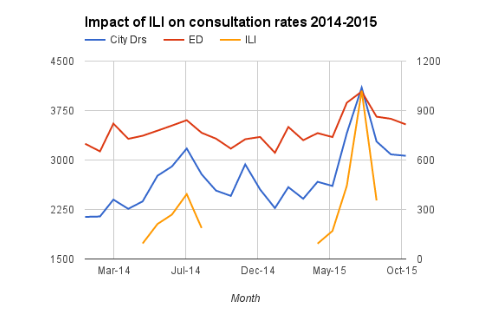
\includegraphics[scale=0.50]{ILI.png}
\caption{The short term impact of Influenza-like-illness on utilization of the Emergency department}
\label{Impact of Influenza-like-illness}
\end{figure}

The utilisation of General Practice by all age groups shows little variation (Figure 13) despite the influenza outbreak and the changes in funding policy. There is the usual winter rise in the 0-4 year age group. There was a non-sustained rise in utilization the 5-14 year age bracket. By December 2015 all age groups had resumed their historic non-winter utilization levels. \\

\begin{figure}[htp]
\centering
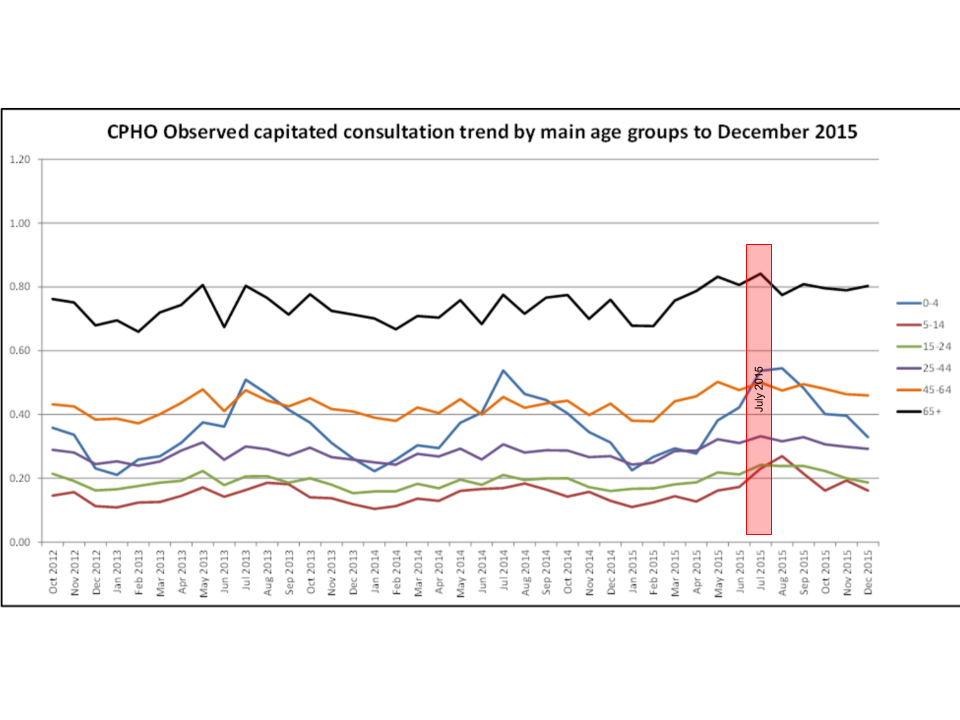
\includegraphics[scale=0.30]{GPu13.png}
\caption{Stratified rates of GP consultations for Central PHO practices}
\label{Age stratified General Practice consultations}
\end{figure}

\subsection{Impacts within ED}
In contract the Emergency Department showed an immediate and sustained effect (Figure 14) that continues far beyond the end of the seasonal influenza outbreak. Indeed Emergency Department utilisation has never returned to historic normal levels.\\

\begin{figure}[htp]
\centering
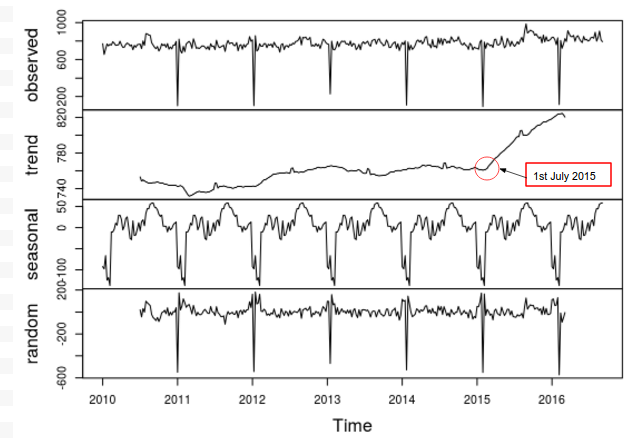
\includegraphics[scale=0.60]{TS_ED.png}
\caption{Time series analysis splitting from all Emergency Department presentations, the changing trends for utilisation from the underlying seasonal patterns.}
\label{Time series analysis of Emergency Department presentations}
\end{figure}

\begin{figure}[htp]
\centering
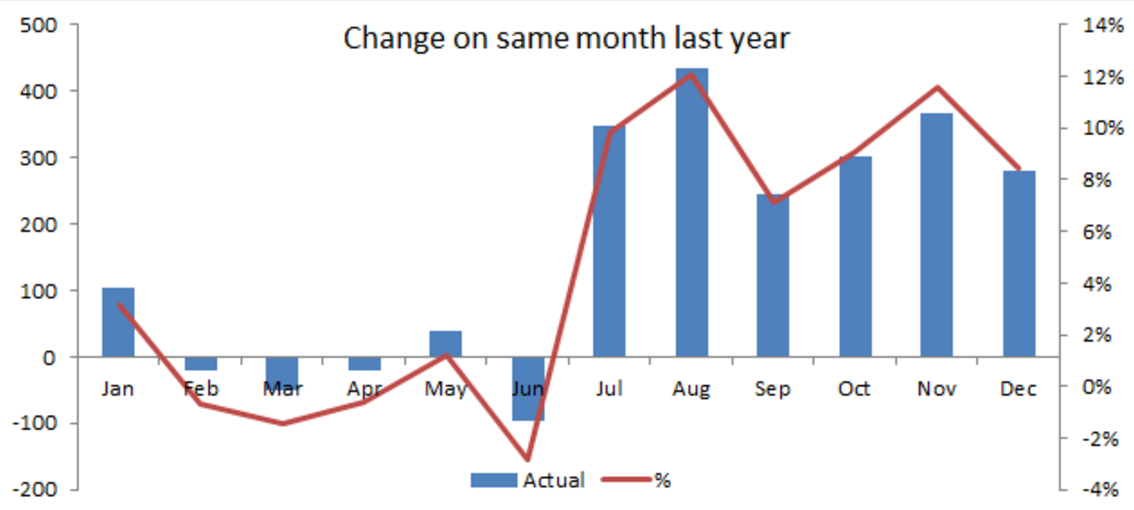
\includegraphics[scale=0.35]{ED.png}
\caption{Comparing 2015 with 2014 showing the relative increase}
\label{Relative changes in ED utilization}
\end{figure}

This change in utilisation patterns is even more marked for those who have used the department for two or three times within the same year.\\

\begin{figure}[htp]
\centering
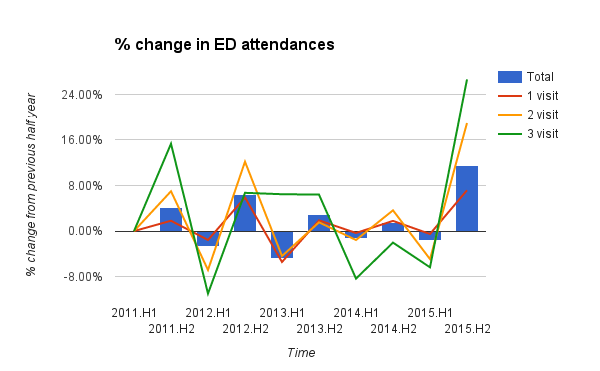
\includegraphics[scale=0.70]{Fchange.png}
\caption{Changes in ED utilisation in H2 2015, especially for rates of second and third time utilisation within the quarter}
\label{Changes in ED utilisation}
\end{figure}

The availability of primary care may be a driving factor, where availability is widely described as the ability to access acute or urgent care either their General Practitioner or via one of the Urgent care facilities. The presentations at ED from the four towns and their associated rural areas was plotted using both Estimated Weighted Moving Average (EWMA) plots and time series plots. The summary of the trends is;\\ 
\\
\\
\begin{tabular}{|l|l|}
\hline 
	Locality & Trend\\
\hline
	Palmerston North & Overall rise since 1.July.2015\\
\hline
	Horowhenua & Initial rise since 1.July.2015 but this has now stabilised\\
\hline
	Tararua & Overall rise since 1.July.2015\\
\hline
	Manawtu (Feilding) & Rise since 2012\\
\hline
\end{tabular}
\\
\\
To further investigate the impact of domicile on ED presentation following the introduction of the free 6-13 year old funding, the rate of presentation by suburb was plotted by suburb. This showed a mixed effect. There was a rise in utilisation by those suburbs who were wealthy and those with proximity to the hospital. Suburbs with high NZDep scores had a mixed result, with some increasing their Emergency Department utilisation, others decreasing.
\pagebreak

\emph{Palmerston North Suburbs}

\begin{tabular}{|l|l|}
\hline
	Suburb & Trend since 1.July.2015\\
\hline
	Kelvin Grove & Rise\\
\hline
	Milson & Rise\\
\hline
	Roslyn & Rise\\
\hline
	Papaeoia & Rise\\
\hline
	Palmerston North Central & Decrease\\
\hline
	Hokowhitu East & No change\\
\hline
	Hokowhitu Lagoon & Rise\\
\hline
	Hokowhitu West & No change\\
\hline
	Awapuni North & Rise\\
\hline
	Awapuni West & No change\\
\hline
	Awapuni South & No change\\
\hline
	Westbrook & No change\\
\hline
	Highbury & Decrease\\
\hline
	Cloverlea & Rise\\
\hline
\end{tabular}
\\
\\

\emph{Ethnicity}

To consider the impact of ethnicity, the same analysis was completed. Again a mixed pattern of results was revealed for ED utilisation.\\

\begin{tabular}{|l|l|}
\hline
	Ethnicity & Trend since 1.July.2015\\
\hline
	Maori & Rise\\
\hline
	NZ European & Rise\\
\hline
	Chinese & Decrease\\
\hline
	Indian & Rise\\
\hline
\end{tabular}
\\
\\
What was not expected was the impact of different utilisation by age groups. The rise in utilisation was greatest in the over 12 year old age groups (see figure 17), when the expectation was of no change in their utilisation of the Palmerston North Hospital Emergency Department.\\
\\
\begin{figure}[htp]
\centering
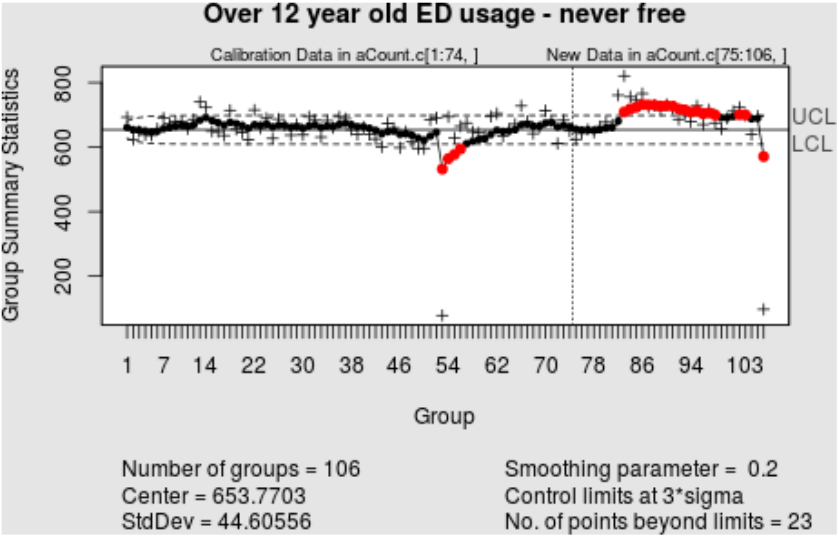
\includegraphics[scale=0.50]{Over12.png}
\caption{EWMA plot showing ED utilisation by those unaffected by funding changes has risen out of control limits}
\label{Rise in ED utilisation by over 12 years old}
\end{figure}
\\

These changes in utilisation has persisted ever since as the new normal (see figure 18).\\
\\

\begin{figure}[htp]
\centering
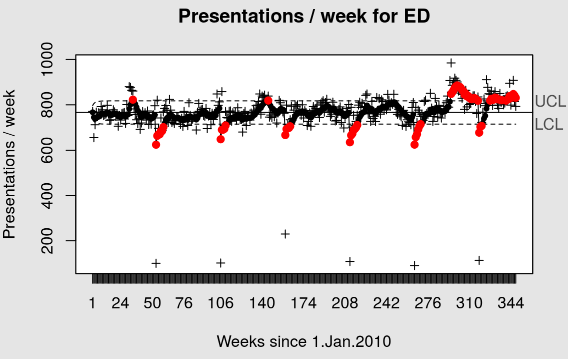
\includegraphics[scale=0.70]{EWMA_ED_pesentations.png}
\caption{EWMA chart of weekly ED presentations since 2010, with weeks put of control limits being displayed in red.}
\label{EWMA statistical process chart of ED presentations}
\end{figure}

and the projections for the future show growth continuing through until 2017, so creating a capacity crisis within the physical Emergency Department.\\

\begin{figure}[htp]
\centering
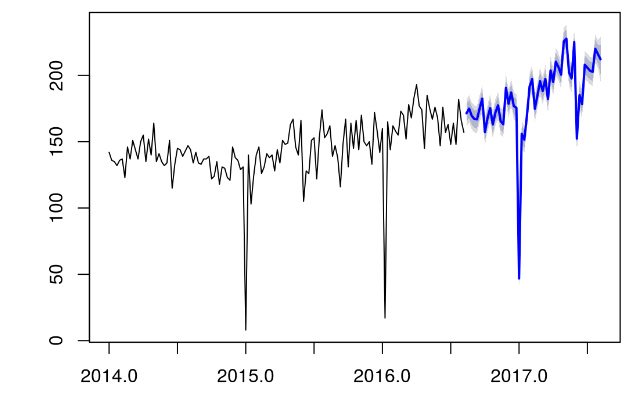
\includegraphics[scale=0.70]{HW_projections.png}
\caption{Projection for ED utilisation using a Holt-Winter's methodology.}
\label{Projections for ED utilisation through to 2017}
\end{figure}

\subsection{Impacts within the Hospital}
Increased demand for hospital based clinical care was a contributor to the poor fiscal result for MidCentral DHB. As increased utilisation of the Emergency Department is associated with increased medical imaging, pharmacy and staff absence due to fatigue so driving upwards the requirements for short term reliefs.\\

\begin{figure}[htp]
\centering
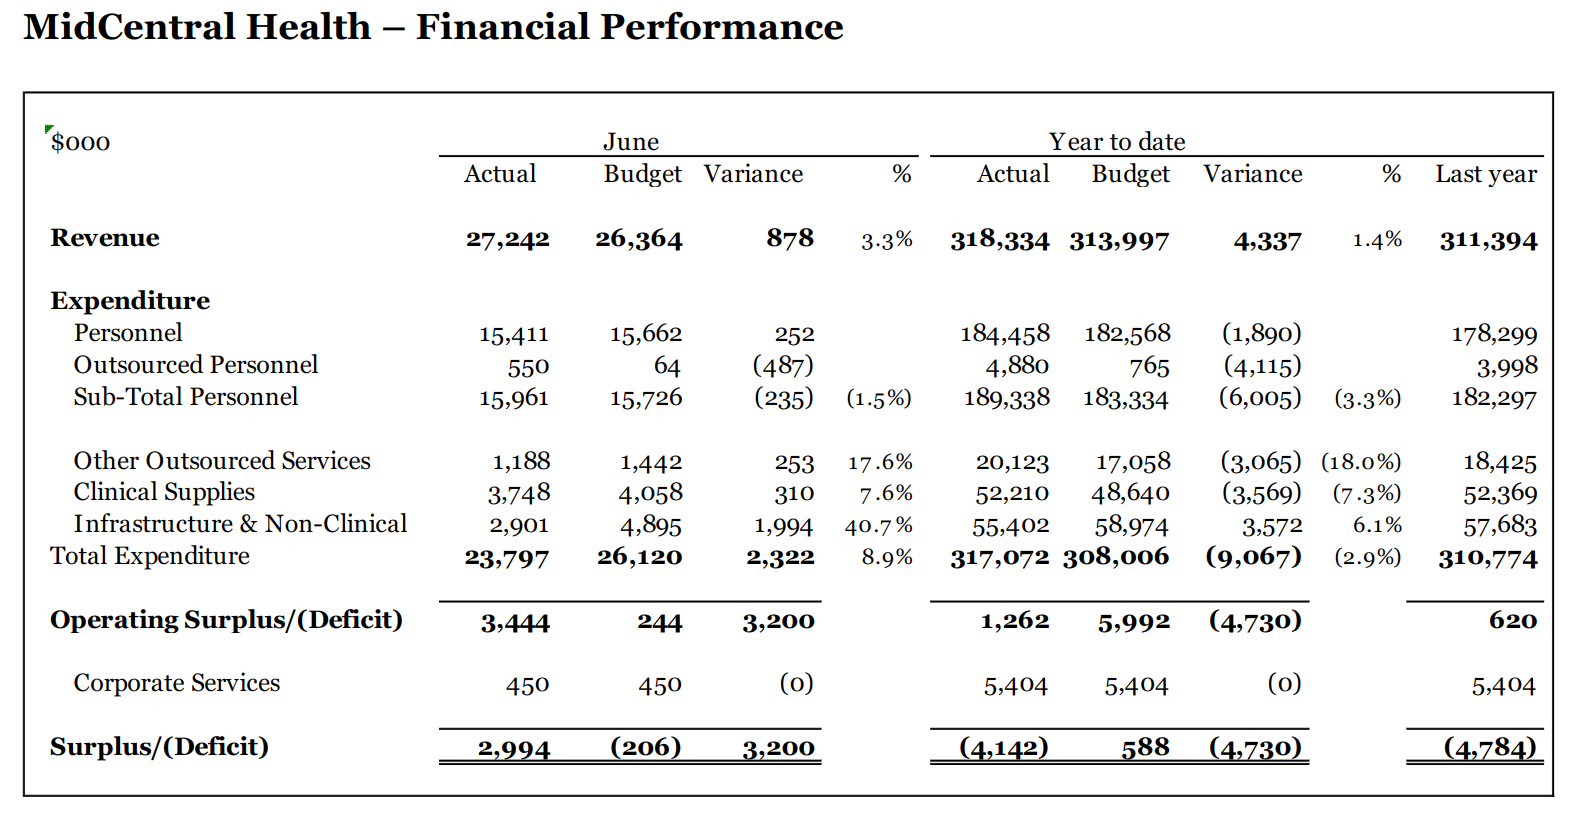
\includegraphics[scale=0.30]{MCHbalance.png}
\caption{Financial result of MidCentral Health or Palmerston North Hospital, showing a significant deficit against budget }
\label{Financial result for MidCentral Health - Palmerston North Hospital}
\end{figure}

\pagebreak

\section{Discussion}
In summary, the use of Game Theory to analyse the results of GIS data enables an understanding of the microeconomic forces consequent to the changes in the macroeconomic policy. In this instance, Game theory analysis supports a proof by abduction that;

\begin{enumerate}
\item The location of primary care and retail outlets in Palmerston North are on almost identical geographical arcs.
\item The location of these arcs is equi-distant between areas of maximal disposable income.
\item Game Theory predicts this equivalence if both are driven by equivalent economic drivers.
\item The distribution of providers is not associated with unmet community need.
\item The distribution of primary care providers is different from services aimed to provide equity of access.
\item There are no local barriers to practices opening in alternative locations.
\end{enumerate}

Hence, in this location primary care provision is a retail activity, not one driven by the need to achieve patient equity or to address unmet patient need. This conclusion is clearly at odds with the objectives of the Primary Health Care strategy and its drive towards equity through increased participation by the disadvantaged. \citet{cumming2008reforming} correctly described how the funding increase was insufficient to break down the financial barriers for participation in the new health market place. Although fees were more affordable on a per annum basis, this is not the same as having sufficient disposable income at the time of need. Those in greatest need need became non-participants in the health system, and were effectively equally spread over all practices. Practices competed for the disposable income of those who could afford the co-payments, as this is the factor that determined practice incomes.\\

This outcome is what Game Theory would predict if the impact of the Primary Care Strategy was to maximise the income from patient co-payment, and not from the capitation payment. Then the practices would align along the Nash equilibrium that was equidistant between areas of maximal disposable income. With hindsight the reforms undertaken within the Primary Health Care Strategy were more idealistic than anticipated. General Practitioners remained steeped in the "fee for service" as a business model. Likewise the patients do not seem to have appreciably changed their behaviour either with regards to service utilisation by still focusing on medical care or by shifting their care paradigm from reactive acute care to preventative chronic care. \\

Currently the "free under 13" policy has had no perceivable impact on General Practitioners. They have not changed their measured consultation patterns, nor has any change in the prevailing Nash equilibrium arc been noted. The later could be due to the relatively short time frame, given it took 15 years for the primary health care strategy to impact practice location. That no change in the consultation patterns across the age range has occurred suggests it has had no impact. This fits with the model that economically General Practice is focused on the patient co-payments, so changes in capitation would not be expected to have any effect in behaviour.\\

The increase Emergency Department utilisation could be coming from those who do not use general practice through economic exclusion or who were unable to register with a practice. What has been built up within the system is a degree of unmet (and potentially unmeetable) need within the community that was unmasked with the fresh funding on 1st.July.2015.\\

Instead ED through improved compliance with the six hour Ministry of health target, has become substantially (time) cheaper and is readily available 24 hours a day, with no financial barriers at all. Hence the rise in utilisation. Given the rise in utilisation by adults unaffected by new funding suggests a social phenomena has also occurred. The expectation has become that health care should be free. It is free for under 13 years, free at the Hospital ED, and should be free elsewhere, or elsewhere seems relatively expensive. \\

The risks from this shift in utilisation patterns is perilous for the DHB. ED is not an infinite resource and there is physical constraints to the building, even if extra emergency department staff can be found. Unless a new building and extra staff is found, then the DHB will default on the compliance with the six hour target. If the DHB does build a new building, it will default on its financial targets and the DHB is currently on performance watch by the Ministry and keen to find a solution \footnote{http://www.stuff.co.nz/manawatu-standard/news/72250866/MidCentral-DHB-on-performance-watch-after-poor-financial-result}. \\

Care in the Emergency Department is not cheap care for the DHB to deliver. Currently the cost is approximately three times the cost of urgent accident related care in an Urgent Care Clinic or about five times the cost of equivalent acute conditions being treated in General Practice. This is before the costs of any unnecessary admissions are considered.\\

An economic model developed under Game Theory therefore can predict the current state. Through the inclusion of practice location within the economic landscape, it provides a more robust model than classic "supply \& demand" economic theory. The question is will this utility persist as the third phase of health sector reforms occurs with the opening of IFHC facilities? The hope is that the formation of the IFHC across the district, will increase the supply of General Practitioners and offer the opportunity for nurses to expand their scope of practice. It could argued that\citet{howell2005restructuring} has been proved to be correct. The size of the business units (the small 2-3 practitioner surgeries) was indeed too small to manage the risks inherent within a capitation model \citep{howell2005restructuring}. Her argument that a formal insurance model involving a larger group of patients is required to provide the risk management associated with an ageing population and shifts in utilisation patterns, is not proven by this study, but seems reasonable. For \citet{howell2005restructuring}, the size of the new IFHC that are opening is more realistic for the insurance based model to enable the achievement of the health reforms envisaged in the primary health care strategy to be achieved.\\

This development may create a paradox. The IFHC that is now large enough to risk manage capitation funding as a basis for funding, allowing capitation funding to become the economic driver that makes care for disadvantaged attractive that it was originally intended to be in the Primary Healthcare strategy \citep{king2001primary}. Indeed capitation funding will be increasingly attractive to IFHC, as growth slows in the co-payment market associated with slow population growth and market saturation for primary care provision to the affluent. The IFHC also face increased cost with new enlarged facilities and the establishment costs of the amalgamations. So while both the need and the opportunity exists, IFHC may struggle to exploit the opportunities. It is not clear is the IFHC are configured to meet the needs or ambitions of the disadvantaged, and they are certainly not located in areas of disadvantage. The IFHC current business model is still centred on maximisation of co-payments and the model of care is configured accordingly. The basis for the assumption that non-participation by the disadvantaged is only due to financial barriers is not clear. The model of care that suits one section of society might not apply to another. Even if the model of care is the same, to exploit the capitation funding opportunity, an IFHC needs to provide some form of outreach into areas of high capitation from their current location in areas of high co-payments to exploit the opportunity.\\

These dilemmas will create economic pressures on existing businesses, so Game theory would predict that the arcs associated with the Nash equilibrium will shift with time. These shifts will reflect changes in IFHC business models including the potential for some to fail if they can not adapt, but also the impact of any new macroeconomic policies or realities will drive shifts. The DHB could base any market interventions it might be contemplating on where they wish those Nash equilibrium arcs to be located in the geographical as well as the economic landscape.\\

For health system planning, the question becomes how to support the IFHC development and exploit the opportunities to improve access to healthcare through the greater relevance of capitation funding in practice income streams. The need is develop a strategy that does not result in misalignment between intentions and reality\citep{kerr1995folly}. Game theory would suggest the focus on community out reach from the IFHC into localities of need, would bridge the gap.\\

\section{Recommendations}
 From this study this report would like to advance the following recommendations for for further consideration;
 
\begin{enumerate}
\item That although this report provides initial support for Game Theory in conjunction with modern data analysis methods as a basis for assessing and planning healthcare delivery, more research is needed.
\item Specifically the study needs to be repeated in another and larger market.
\item The study needs to be repeated with a more robust and comprehensive data set.
\item The study needs to be longitudinal given the long time frames for changes within primary care impacting on the business models of owners.
\item MidCentral DHB needs to consider how it will meet the needs of the disadvantaged or those that live in areas of high need. Consideration may be given to opening a medical centre in such an area. It will be important that barriers to capture by the affluent are set in place. If the health centre was a welfare centre established as a joint venture with Ministries of Housing \& Social Welfare then the rules of the "game" would be different from those seen at the IFHC or General Practices within Palmerston North.
\item MidCentral DHB needs to consider changing the paradigm of primary and secondary care being separate entities. Events in once cause negative impacts in the other. These issues can only be addressed through adopting a whole of sector management strategy. 
\end{enumerate}
\pagebreak

\section{Postscript}
The last outlying medium practice not conforming to the model previously has just announced that as it is moving. The current site was found to be uneconomic and they are moving onto the same zone of maximal access to affluence as all other medium to large practices. These business decisions are as predicted by the Nash equilibrium model of local primary care delivery. \\

Two of the remaining solo practitioners have retired and their practices folded into an IFHC. These leaves only two solo-practitioners who are non-conforming to the model described in this report. Neither of whom are principally driven by economic factors in their business decisions, so their business decisions are not "rational" from an economic perspective so are not predictable by this methodology.\\ 

\pagebreak

\bibliography{report.bib}
\end{document}

